Evaluation took the form of a user study, in which we provided a directed walkthrough of our work to novice users, after which we asked a nine linear scale questions about their experience.
We walked users through as follows:

\begin{enumerate}
    \item The user was briefed on the purpose of the project, and that the end effector would be be their point of interaction with the terrain, both for painting and for feedback.
    \item The user was directed through the menu and setup screens.
    \item The user was shown the texture selection menu and told to paint different textures.
    \item The user was allowed to explore this functionality to their satisfaction.
    \item The user was shown the object selection menu and told to paint different objects.
    \item The user was allowed to explore this functionality to their satisfaction.
    \item The user was shown the object deletion menu and told to delete existing objects.
    \item The user was allowed to explore this functionality to their satisfaction.
\end{enumerate}

After this experience, the user was asked the following set of nine 5-point linear scale questions, and told to answer between 5 meaning "most" and 1 meaning "least":
\begin{enumerate}
    \item How easy was it to tell the difference between feedback from objects and feedback from surface textures?
    \item How easy was it to tell the difference between feedback from different surface textures?
    \item How easy was it to tell the difference between feedback from different objects?
    \item How easy was it to tell the difference between feedback from all sources at different zoom levels?
          \vspace{3mm}
    \item How helpful was feedback from objects in understanding and navigating the current state of the terrain?
    \item How helpful was feedback from texture in understanding and navigating the current state of the terrain?
          \vspace{3mm}
    \item How synchronized was haptic feedback with the terrain you saw on screen?
    \item How physically fatiguing did you find the haptic feedback?
    \item How would you rate your overall enjoyment of the experience?
\end{enumerate}

\begin{figure}
    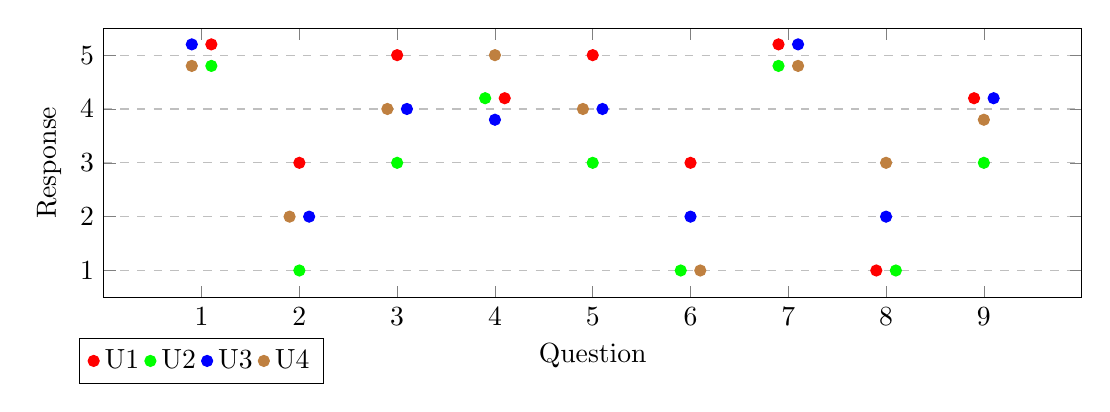
\begin{tikzpicture}
        \begin{axis}[
                width=14cm,
                height=5cm,
                xlabel={Question},
                ylabel={Response},
                xmin=0, xmax=10,
                ymin=0.5, ymax=5.5,
                xtick={1,2,3,4,5,6,7,8,9},
                ytick={1,2,3,4,5},
                legend pos=north west,
                ymajorgrids=true,
                grid style=dashed,
                legend columns=8,
                legend style={at={(0.1,-0.15)},anchor=north}
            ]
            \addplot[only marks, color=red]
            coordinates{(1.1,5.2)(2,3)(3,5)(4.1,4.2)(5,5)(6,3)(6.9,5.2)(7.9,1)(8.9,4.2)};
            \addlegendentry{U1}

            \addplot[only marks, color=green]
            coordinates{(1.1,4.8)(2,1)(3,3)(3.9,4.2)(5,3)(5.9,1)(6.9,4.8)(8.1,1)(9,3)};
            \addlegendentry{U2}

            \addplot[only marks, color=blue]
            coordinates{(0.9,5.2)(2.1,2)(3.1,4)(4,3.8)(5.1,4)(6,2)(7.1,5.2)(8,2)(9.1,4.2)};
            \addlegendentry{U3}

            \addplot[only marks, color=brown]
            coordinates{(0.9,4.8)(1.9,2)(2.9,4)(4,5)(4.9,4)(6.1,1)(7.1,4.8)(8,3)(9,3.8)};
            \addlegendentry{U4}
        \end{axis}
    \end{tikzpicture}
    \caption{User Study Responses}
    \label{fig:user-study}
\end{figure}

The responses to these questions is charted in \autoref{fig:user-study}; we provide data on four respondents, grouped by color. Overall sentiment was positive with respect to force feedback, with all respondents rating both the utility and differentiability of shape-driven feedback highly.
Users generally found it difficult to differentiate between textures, and did not find them helpful for terrain navigation. We conjecture improving texture differentiability would improve the usefulness of this feedback, though in its current state textural feedback still provides users feedback on scale and rate of motion. Users did however find it easy to discriminate scale on the basis of haptic feedback.
Users generally did not find the experience fatiguing, and found it both well-synchronized with the visual terain rendering and enjoyable overall.

We conclude that users generally felt that feedback from scene objects was both salient and useful, but that textures fell short due to difficulty in differentiation. However, the positive responses for both sentiment, fatigue, and usefulness of shape-driven feedback supports the viability of the project.